\section{Complex Numbers}
\begin{namedframe}{What is an Imaginary Number?}
	\begin{center}
		Usually, we work with \textit{real} numbers. \\
		Real include all integers, rational numbers, and irrational numbers. \\
		e.g. $1,\ 6.9,\ \pi,\ e,\ \sqrt{123}$
	\end{center}

	\begin{block}{Definition of i}
		$\imagi$ is defined as $\sqrt{-1}$. \\
		$\therefore \imagi^2 = -1; (-\imagi)^2 = -1$
	\end{block}
\end{namedframe}

\begin{namedframe}{What is a Complex Number?}
	\begin{block}{Definition of a complex number}
		A complex number is the sum of a real and imaginary number.
	\end{block}

	\begin{center}
		e.g. $1 + \imagi,\ \pi + ei,\ 0 + \imagi,\ 1 + 0\imagi$, etc
	\end{center}

	Complex numbers have interesting properties, including how
	they and, multiply, and exponentiate.
\end{namedframe}

\begin{namedframe}{Adding and Subtracting Complex Numbers}
	You can add and subtract complex numbers like you would add polynomials (combine like terms).
	\begin{exampleblock}{Example 1}
		\[(5 + 3\imagi) + (6 + 4\imagi) = 11 + 7\imagi\]
	\end{exampleblock}

	\begin{exampleblock}{Example 2}
		\[(3 + 6\imagi) - (6 - 4\imagi) = -3 + 2\imagi\]
	\end{exampleblock}
\end{namedframe}

\begin{namedframe}{Conjugates and Magnitudes}
	For some complex number $a + bi$, its \textbf{conjugate} is $a - bi$. \\
	The conjugate of a complex number $z = a + bi$ is denoted with $\overline{z}$.
	\begin{exampleblock}{Example}
		What is the conjugate of $3 + 5\imagi$?
		\pause
		\[3 - 5\imagi\]
	\end{exampleblock}

	\pause

	For some complex number $a + bi$, its \textbf{magnitude} is $a^2 + b^2$. \\
	The magnitude of a complex number $z = a + bi$ is denoted with $|z|$.
	\begin{exampleblock}{Example}
		What is the magnitude of $3 + 5\imagi$? \\
		\pause
		\phantom{X}$3^2 + 5^2$ \\
		$ = 34$
	\end{exampleblock}
\end{namedframe}

\begin{namedframe}{Multiplying Complex Numbers}
	You can multiply complex numbers like you would multiply binomials (using FOIL).
	\begin{exampleblock}{Example}
		If $a = 5 + 3\imagi$ and $b = 6 + 4\imagi$, then \\
		$\phantom{X}(5 + 3\imagi)\times(6 + 4\imagi)$ \\
		$= (5\times6) + (5\times4\imagi) + (3\imagi\times6) + (3\imagi\times4\imagi)$ \\
		$= 30 + 20\imagi + 18\imagi + 12\imagi^2$ \\
		$= 30 + 38\imagi - 12$ \\
		$= 18 + 38\imagi$ \\
	\end{exampleblock}
\end{namedframe}

\begin{namedframe}{Multiplying Complex Numbers}
	A complex number multiplied by its conjugate always gives its magnitude.
	\begin{exampleblock}{Example}
		$\phantom{X}(5 + 3\imagi)\times(5 - 3\imagi)$ \\
		$= 5^2 - (3\imagi)^2$ \\
		$= 34$
	\end{exampleblock}
\end{namedframe}

\begin{namedframe}{Dividing Complex Numbers}
	To divide complex numbers, make the denominator into a real number by multiplying top
	and bottom by its conjugate.
	\begin{exampleblock}{Example}
		$\dfrac{1 + 2\imagi}{2 - 3\imagi}$ \\
		$ = \dfrac{(1 + 2\imagi)(2 + 3\imagi)}{(2 - 3\imagi)(2 + 3\imagi)}$ \\
		$ = \dfrac{2 + 3\imagi + 4\imagi + 6\imagi^2}{2^2 - (3\imagi)^2}$ \\
		$ = \dfrac{-4 + 7\imagi}{13}$ \\
		$ = \dfrac{-4}{13} + \dfrac{7}{13}\imagi$ \\
	\end{exampleblock}
\end{namedframe}

\begin{namedframe}{Dividing Complex Numbers}
	The general formula for dividing complex numbers $a$ by $b$ is:
	\begin{block}{Formula}
		\[\dfrac{a \times \overline{b}}{|b|}\]
	\end{block}
\end{namedframe}

\begin{namedframe}{Complex Plane}
	Complex points can be visualized on the complex plane.
	\begin{center}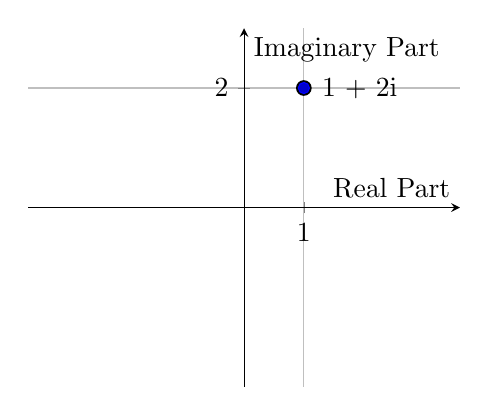
\begin{tikzpicture}\begin{axis}[
		xlabel=Real Part,
		ylabel=Imaginary Part,
		axis lines=middle,
		axis equal,
		grid=both,
		xmin=-3,
		ymin=-3,
		xmax=3,
		ymax=3,
		xtick=1,
		ytick=2,
		scale=0.8
	]
		\addplot coordinates{(1, 2)};
		\node[label={0:{1 + 2i}},circle,fill,inner sep=2pt] at (axis cs:1,2) {};
	\end{axis}\end{tikzpicture}\end{center}
	\pause
	The \textbf{magnitude} of the number is the distance of the point from the origin. \\
	The \textbf{argument} is the polar angle (angle counter-clockwise from the x-axis in the positive direction)
	of the point.
\end{namedframe}

\begin{namedframe}{Conversion}
	Converting $a + bi$ form to and from magnitude-argument (\textbf{polar}) form requires some trigonometry.
	\begin{block}{$a + bi$ form to polar form}
		Magnitude = $|z| = a^2 + b^2$ \\
		Argument = $arg(z) = atan2(a, b)$ \\
		% Stolen from Wikipedia
		$atan2(y,x)=\begin{cases}\arctan({\frac {y}{x}})&{\text{if }}x>0,\\\arctan({\frac {y}{x}})+\pi &{\text{if }}x<0{\text{ and }}y\geq 0,\\\arctan({\frac {y}{x}})-\pi &{\text{if }}x<0{\text{ and }}y<0.\end{cases}$ \\
		\footnotesize 
	\end{block}
	\footnotesize
	(\LaTeX code stolen from Wikipedia) \\
	\normalsize
	The atan2 formula is derived from CAST rule.
\end{namedframe}

\begin{namedframe}{Conversion}
	Converting $a + bi$ form to and from magnitude-argument (\textbf{polar}) form requires some trigonometry.
	\begin{block}{Polar form to $a + bi$ form}
		Where $Re(z)$ is the real part of the complex number and $Im(z)$ is the imaginary part of the complex number \\
		and $\theta = \arg(z)$,
		\[Re(z) = |z| \times \cos(\theta)\]
		\[Im(z) = |z| \times \sin(\theta)\]
	\end{block}
\end{namedframe}

\begin{namedframe}{Euler's Formula}
	Given a complex number in polar form, it can also be written in a closed-form expression (without converting back to $a + bi$).
	\begin{block}{Euler's Formula}
		For some complex number $z$: \\
		$z = |z| \times e^{arg(z) \times \imagi}$
	\end{block}

	\tiny
	Anecdote: Within a certain set of people, whenever someone says "Euler's Formula" or "Euler's Theorem",
	another person always asks "which one?". It occurred to be that while this was not just a joke; we actually
	need clarification because we have at some point or another mentioned this formula, Euler's Formula about
	planar graphs, and the Euler-Fermat Theorem.
\end{namedframe}

\begin{namedframe}{Exponentiation with Complex Numbers}
	De Moivre's Formula gives us a useful way of exponentiating complex numbers in polar form.
	\begin{block}{Statement}
		For some complex number $z$ and integer $n$, if $y = z^n$, \\ 
		\[y| = |z|^n\] \\
		\[arg(y) = arg(z) \times n\] \\
		Less formally, a complex number raised to the $n^{\text{th}}$ power has its magnitude
		raised to the $n^{\text{th}}$ power and its argument multiplied by $n$.
	\end{block}

	This can be trivially proven with Euler's Formula.
\end{namedframe}
